\documentclass[11pt,a4paper]{article}

% ----- Page layout -----
\usepackage[a4paper,margin=2.5cm]{geometry}
\usepackage{parskip}
\usepackage{microtype}

% ----- Math -----
\usepackage{amsmath,amssymb,amsfonts}
\usepackage{mathtools}
\usepackage{bm}
\usepackage{siunitx}
  \sisetup{per-mode=symbol, separate-uncertainty=true}

% ----- Graphics & figures -----
\usepackage{graphicx}
\usepackage{float}
\usepackage{caption}
\captionsetup{font=small,labelfont=bf,skip=4pt}
\usepackage{subcaption}

% ----- TikZ / CircuiTikZ -----
\usepackage{tikz}
\usepackage{circuitikz}
\usetikzlibrary{calc,arrows.meta,positioning}

% ----- Tables -----
\usepackage{booktabs}
\usepackage{array}
\usepackage{tabularx}

% ----- Headers, hyperlinks, colors -----
\usepackage{xcolor}
\usepackage{hyperref}
\hypersetup{colorlinks=true,linkcolor=blue!60!black,urlcolor=blue!60!black,citecolor=blue!60!black}
\usepackage{enumitem}
\usepackage{fancyhdr}
\pagestyle{fancy}
\fancyhf{}
\fancyhead[L]{\small ET4260 -- Microsystems Design and Modelling}
\fancyhead[R]{\small Homework Unit 4\&5}
\fancyfoot[C]{\thepage}
\renewcommand{\headrulewidth}{0.4pt}

% ----- Section coloring to match the assignment "Part X" banners -----
\usepackage{titlesec}
\definecolor{tudblue}{RGB}{0,118,194}
\titleformat{\section}{\Large\bfseries\color{tudblue}}{}{0pt}{}[{\titlerule[0.8pt]}]

\newcommand{\LWeff}{\left(\tfrac{L}{W}\right)_{\!\mathrm{eff}}}

\begin{document}

% ===================== Title page =====================
\begin{titlepage}
\centering
\vspace*{1cm}
{\large\textbf{DELFT UNIVERSITY OF TECHNOLOGY}}\\[2pt]
{\small Faculty of Electrical Engineering, Mathematics and Computer Science}\\[2cm]

\includegraphics[width=0.25\textwidth]{figures/tudelft_logo.jpeg}\\[2cm]
{\Large\textbf{Homework Unit 4\&5 (ET4260) 2026}}\\[6pt]
{\Large\textbf{Semiconductor Sensors \&}}\\[4pt]
{\Large\textbf{Introduction to Finite Element Modelling}}\\[1.5cm]

\begin{minipage}{0.85\textwidth}
\centering\small
\textbf{Instructions.} Document your calculations properly with derivations and screenshots when needed. Submission in Word or PDF format.
\end{minipage}
\vfill
\rule{0.7\textwidth}{0.4pt}\\[4pt]
{\large Daniel Tyukov}\\[2pt]
{\large Student number: 5714699}\\[4pt]
\rule{0.7\textwidth}{0.4pt}
\vspace{1cm}
\end{titlepage}

\section*{Part A: Hall Sensors}
\addcontentsline{toc}{section}{Part A: Hall Sensors}

\paragraph{Task 1 a) Best intrinsic semiconductor.}
The current-related sensitivity of a Hall plate is $S_I = rG/(n\,q\,t)$ and the voltage-related
sensitivity is $S_V = \mu\,rG/\LWeff$. For an intrinsic material $n=n_i$, so a good Hall sensor
wants a \emph{low} intrinsic carrier concentration and a \emph{high} mobility. Reading Table~1:

\begin{center}\small
\begin{tabular}{lccc}
\toprule
 & Si & GaAs & Ge \\
\midrule
$n_i$ [\si{\per\cubic\cm}] & $1.5\times10^{10}$ & $\bm{1.8\times10^{6}}$ & $2.4\times10^{13}$ \\
$\mu_n$ [\si{\square\cm\per\volt\per\second}] & 1350 & \textbf{8500} & 3900 \\
\bottomrule
\end{tabular}
\end{center}

GaAs wins on \emph{both} counts: its intrinsic concentration is four orders of magnitude below Si
(boosting $S_I\propto 1/n_i$) and its electron mobility is the highest of the three (boosting
$S_V\propto\mu$). Its wide bandgap (\SI{1.42}{eV}) also keeps thermally generated carriers low, so
the response stays stable with temperature. \textbf{GaAs is the most suitable.}

\paragraph{Task 1 b) Parameter linking $S_I$ and $S_V$.}
Since $V=I\!\cdot\!R$, the two sensitivities are tied through the \textbf{device resistance $R$}:
\[
S_V=\frac{S}{V}=\frac{S}{I R}=\frac{S_I}{R},\qquad R=R_\square\LWeff .
\]
$R$ matters in its own right because it fixes the bias power $P=V^2/R=I^2R$ (hence self-heating) and
the thermal-noise floor $\overline{u_n^2}=4k_BTR\,\Delta f$. Designing only for sensitivity while
ignoring $R$ can push the device into excessive power dissipation or poor SNR.

\paragraph{Task 1 c) Figure of merit for integrated devices.}
An integrated Hall device runs from a fixed supply \emph{voltage} and a limited power budget, so the
\textbf{voltage-related sensitivity $S_V$} (\si{\volt\per\volt\per\tesla}) is the meaningful figure of
merit, since it is the sensitivity per unit bias and ultimately sets the achievable SNR-per-power,
$\mathrm{SNR}_P\propto \mu\,rG/\LWeff$.

\paragraph{Task 1 d) GaN Hall devices.}
For the Gen~2 device $S_I=\SI{90}{\volt\per\ampere\per\tesla}$, $S_V=\SI{57}{\milli\volt\per\volt\per\tesla}$,
$R_\square=\SI{430}{\ohm}/\square$, with $r=1$.

\textbf{(i)} From $S_V=S_I/\big(R_\square\LWeff\big)$,
\[
\LWeff=\frac{S_I}{S_V\,R_\square}=\frac{90}{0.057\times430}=\mathbf{3.67}.
\]
The geometry factor follows from
\[
G\approx\frac{\LWeff^{2}}{\sqrt{\LWeff^{4}+\tfrac12\LWeff^{2}+4}}
=\frac{3.67^{2}}{\sqrt{3.67^{4}+\tfrac12\,3.67^{2}+4}}=\mathbf{0.97}.
\]
($G$ is close to unity, as expected for the relatively large $L/W$ of a cross/Greek-cross plate.)

\textbf{(ii)} Gen~3 shares Gen~2's geometry, so $\LWeff=3.67$ and $G=0.97$ carry over. With
$S_I=34$, $S_V=\SI{34}{\milli\volt\per\volt\per\tesla}$,
\[
R_{\square,\mathrm{Gen3}}=\frac{S_I}{S_V\LWeff}=\frac{34}{0.034\times3.67}=\mathbf{272\ \si{\ohm}/\square}.
\]

\textbf{(iii)} Sheet carrier density from $S_I=rG/(n_s q)$ and mobility from $S_V=\mu rG/\LWeff$:
\[
n_s=\frac{rG}{S_I\,q},\qquad \mu=\frac{S_V\LWeff}{rG}.
\]

\begin{center}\small
\begin{tabular}{lccc}
\toprule
 & $n_s=n\!\cdot\!t$ [\si{\per\square\cm}] & $\mu$ [\si{\square\cm\per\volt\per\second}] & cross-check $\mu=1/(R_\square q n_s)$ \\
\midrule
Gen~2 & $6.74\times10^{12}$ & $2154$ & \SI{2154}{} \checkmark\\
Gen~3 & $1.78\times10^{13}$ & $1285$ & \SI{1285}{} \checkmark\\
\bottomrule
\end{tabular}
\end{center}

Gen~3's InAlN barrier gives a roughly $2.6\times$ higher 2DEG density but a lower mobility, the
usual density/mobility trade-off in nitride heterostructures.

\textbf{(iv) Additional: silicon comparison} ($\LWeff=\sqrt2$, so
$G=2/\sqrt{4+1+4}=2/3=0.67$; $S_I=300$, $S_V=\SI{60}{\milli\volt\per\volt\per\tesla}$):
\[
R_{\square,\mathrm{Si}}=\frac{300}{0.060\sqrt2}=\mathbf{3536\ \si{\ohm}/\square},\qquad
n_s=\frac{0.67}{300\,q}=1.39\times10^{12}\,\si{\per\square\cm},
\]
\[
\mu_{\mathrm{Si}}=\frac{0.060\sqrt2}{0.67}=\mathbf{1273\ \si{\square\cm\per\volt\per\second}}.
\]
The Si plate has $\sim$\,8$\times$ the sheet resistance of GaN Gen~2 and only $\sim$\,60\% of its
mobility. GaN therefore delivers both a lower $R_\square$ (more current at fixed power) and a higher
mobility, which is exactly why it makes the better integrated Hall material.

\section*{Part B: Temperature Sensors}
\addcontentsline{toc}{section}{Part B: Temperature Sensors}

\paragraph{Task 3 a) Bias-related sensitivity of the bridge.}
With $V_B$ at the top, the left arm is $R_1$ (top)\,$+$\,$R_3$ (bottom) and the right arm is
$R_2$\,$+$\,$R_4$; the output is $V_o=V_A-V_C$ across the two mid-nodes. The figure pairs
opposite-TCR resistors in adjacent arms ($R_1,R_4$ negative; $R_2,R_3$ positive), which is the
fully-active configuration. Writing $R_n=R(1+\alpha_{\mathrm{neg}}\Delta T)$ and
$R_p=R(1+\alpha_{\mathrm{pos}}\Delta T)$,
\[
V_o=V_B\!\left[\frac{R_3}{R_1+R_3}-\frac{R_4}{R_2+R_4}\right]
   =V_B\,\frac{(\alpha_{\mathrm{pos}}-\alpha_{\mathrm{neg}})\,\Delta T}{2+(\alpha_{\mathrm{pos}}+\alpha_{\mathrm{neg}})\,\Delta T}.
\]
The bias-related sensitivity is the output per unit bias per kelvin, evaluated at balance
($\Delta T\!\to\!0$):
\[
S_{\mathrm{bias}}=\frac{1}{V_B}\frac{\partial V_o}{\partial T}\bigg|_{0}
=\frac{\alpha_{\mathrm{pos}}-\alpha_{\mathrm{neg}}}{2}
=\frac{5\times10^{-4}-(-3\times10^{-4})}{2}
=\mathbf{4\times10^{-4}\ \si{\per\kelvin}}\;(=\SI{0.4}{\milli\volt\per\volt\per\kelvin}).
\]

\paragraph{Task 3 b) SNR vs.\ temperature.}
\textbf{Signal:} the output grows essentially linearly with $\Delta T$,
$V_o\approx V_B(\alpha_{\mathrm{pos}}-\alpha_{\mathrm{neg}})\Delta T/2$, and is \emph{zero} at the
balance point $T_0$. \textbf{Noise:} the dominant term is the thermal noise of the bridge's output
resistance, $u_n=\sqrt{4k_BT\,R_{\mathrm{out}}\,\mathrm{ENBW}}$, which depends only weakly on
temperature. For the symmetric case $\alpha_{\mathrm{neg}}=-\alpha_{\mathrm{pos}}$ the two TCRs
cancel in $R_{\mathrm{out}}$, so $R_{\mathrm{out}}\approx R$ stays constant and the only temperature
dependence of the noise is the slow $\sqrt{T}$. Hence
\[
\mathrm{SNR}=\frac{V_o}{u_n}\propto\frac{\Delta T}{\sqrt{T}} .
\]
The SNR is zero at $T_0$ and \emph{increases monotonically} as the temperature moves away from
balance, because the numerator climbs linearly while the noise rises only as $\sqrt{T}$.

\textbf{Additional task: exact SNR.} Using the exact $V_o(T)$,
$R_{\mathrm{out}}=2R_nR_p/(R_n+R_p)$ and $u_n=\sqrt{4k_BT\,R_{\mathrm{out}}\,\mathrm{ENBW}}$ with
$V_B=\SI{5}{\volt}$, $R=\SI{1}{\kilo\ohm}$, $\mathrm{ENBW}=\SI{1}{\kilo\hertz}$ and the part-a)
$\alpha$-values gives Fig.~\ref{fig:snr}. The curve rises from $-\infty$ at the \SI{300}{\kelvin}
balance point to about \SI{122}{dB} at \SI{400}{\kelvin}.

\begin{figure}[H]
\centering
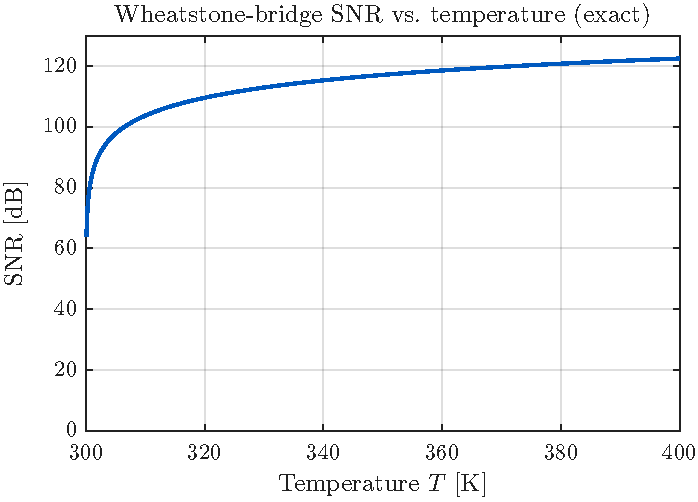
\includegraphics[width=0.62\textwidth]{figures/q3b_snr.pdf}
\caption{Exact Wheatstone-bridge SNR over \SIrange{300}{400}{\kelvin}. The output (and hence the
SNR) vanishes at the \SI{300}{\kelvin} balance point and grows steadily as $|\Delta T|$ increases.}
\label{fig:snr}
\end{figure}

\paragraph{Task 3 c) Measures for sufficient SNR (Additional).}
The problem is the dead zone near $T_0$, where $V_o\to0$. Practical fixes:
\begin{itemize}[nosep,leftmargin=1.4em]
\item \textbf{Offset the bridge} (unbalance it deliberately, e.g.\ trim one arm) so $V_o\neq0$ at the
low end. \emph{$+$} removes the dead zone; \emph{$-$} costs dynamic range and adds offset drift.
\item \textbf{Raise the bias $V_B$:} $\mathrm{SNR}\propto V_B$ while thermal noise is independent of
it. \emph{$+$} direct gain; \emph{$-$} power $\propto V_B^2$ $\Rightarrow$ self-heating error.
\item \textbf{Reduce ENBW / average longer:} noise $\propto\sqrt{\mathrm{ENBW}}$. \emph{$+$} cheap SNR;
\emph{$-$} slower measurement (energy $\times$ time trade-off).
\item \textbf{Higher-TCR materials} (larger $\alpha_{\mathrm{pos}}-\alpha_{\mathrm{neg}}$).
\emph{$+$} more signal; \emph{$-$} worse nonlinearity, needs polynomial correction.
\end{itemize}

\section*{Part C: Photodetectors}
\addcontentsline{toc}{section}{Part C: Photodetectors}

\paragraph{Task 2 a) Absorption, thickness and quantum efficiency.}
\textbf{(i)} Beer--Lambert absorption is $1-e^{-\alpha d}$, so $d=\ln\!\big(\tfrac{1}{1-A}\big)/\alpha$
with $A=0.90$ ($\alpha d=\ln10=2.303$) or $A=0.99$ ($\alpha d=\ln100=4.605$):

\begin{center}\small
\begin{tabular}{lcc}
\toprule
& $d_{90\%}$ & $d_{99\%}$ \\
\midrule
\SI{600}{\nm} ($\alpha=\SI{4140}{\per\cm}$)   & \SI{5.56}{\micro\meter} & \SI{11.1}{\micro\meter} \\
\SI{400}{\nm} ($\alpha=\SI{95200}{\per\cm}$)  & \SI{242}{\nm}           & \SI{484}{\nm} \\
\bottomrule
\end{tabular}
\end{center}
The strongly absorbed blue light (\SI{400}{\nm}) is collected within half a micron, whereas red
light (\SI{600}{\nm}) needs a $\sim$\,20$\times$ thicker active layer.

\textbf{(ii)} Going from the $90\%$ to the $99\%$ thickness, the absorbed fraction rises $0.90\to0.99$,
so the relative change in quantum efficiency is
\[
\frac{\Delta\eta}{\eta}=\frac{0.99-0.90}{0.90}=+10\%,
\]
\emph{identical for both wavelengths}. Roughly doubling the thickness buys only $10\%$ more
efficiency, so the returns diminish quickly.

\textbf{(iii)} With $\eta=(1-\mathcal R)(1-e^{-\alpha d})\zeta$, $\zeta=1$ and $(1-e^{-\alpha d})=0.99$:
\[
\eta(\SI{400}{\nm})=(1-0.485)(0.99)=\mathbf{51.0\%},\qquad
\eta(\SI{600}{\nm})=(1-0.354)(0.99)=\mathbf{63.9\%}.
\]
Red light reaches a higher external efficiency here purely because its surface reflectivity is lower.

\paragraph{Task 2 b) Integrated photoconductor.}
$N_D=\SI{1e17}{\per\cubic\cm}$ ($n=N_D$), $\mu_n=\SI{700}{\square\cm\per\volt\per\second}$,
$\mu_p=\SI{240}{\square\cm\per\volt\per\second}$, $t=\SI{1}{\micro\meter}$, $W=\SI{10}{\micro\meter}$,
$L=\SI{30}{\micro\meter}$, $V=\SI{1.8}{\volt}$.

\textbf{(i) Dark current.} The well is strongly $n$-type ($p=n_i^2/n\approx\SI{2e3}{\per\cubic\cm}$ is
negligible), so $\sigma=nq\mu_n=\SI{11.21}{\siemens\per\cm}$ and
\[
R=\frac{1}{\sigma}\frac{L}{Wt}=\frac{1}{11.21}\cdot\frac{30}{10\times1}\times10^{4}\ \si{\ohm}
 =\SI{2675}{\ohm},\qquad
I_{\mathrm{dark}}=\frac{V}{R}=\mathbf{0.67\ \si{\milli\ampere}}.
\]

\textbf{(ii) Photocurrent.} The photon flux is $\Phi=\phi\,LW=10^{16}\times(30\times10\times10^{-12})
=\SI{3e6}{\per\second}$. The transit time is
$\tau_e=L^2/(\mu_n V)=(\SI{3e-3}{\cm})^2/(700\times1.8)=\SI{7.14}{\nano\second}$, giving a gain
$G=(\tau/\tau_e)(1+\mu_p/\mu_n)=14.0\times1.343=18.8$ (Task~2~b~iii). Hence
\[
i_p=e\,\eta\,\Phi\,G=(1.602\times10^{-19})(0.515)(3\times10^{6})(18.8)=\mathbf{4.65\ \si{\pico\ampere}}.
\]
(The primary photocurrent without recirculation would be $e\eta\Phi=\SI{0.25}{\pico\ampere}$.)

\textbf{(iii) Gain and its geometry dependence.} Combining the expressions,
\[
G=\frac{\tau\,V\,(\mu_n+\mu_p)}{L^{2}}\;\propto\;\frac{1}{L^{2}},\quad\text{independent of }W.
\]
$G=\mathbf{18.8}$. (a) Doubling the length ($2L$) makes $\tau_e$ four times longer, so
$G\to G/4=4.7$. (b) Doubling the width ($2W$) leaves the gain \emph{unchanged}.

\textbf{(iv) Photocurrent for those cases.} Since $\Phi=\phi LW$ scales with area,
$i_p=e\eta\Phi G\propto LW/L^{2}=W/L$:
\[
\text{(a) }2L:\ i_p\to\tfrac12 i_p \ \text{(area }\times2,\ G\times\tfrac14)\,;\qquad
\text{(b) }2W:\ i_p\to 2\,i_p\ \text{(area }\times2,\ G\text{ unchanged).}
\]
Widening the device is the productive way to collect more photocurrent; lengthening it actually
reduces it because the gain loss outpaces the larger collection area.

\section*{Part D: IS-MOS Capacitance}
\addcontentsline{toc}{section}{Part D: IS-MOS Capacitance}

\paragraph{Task 4 a) Labelling and characteristic parameters.}
The curve is a low-frequency MOS C--V on a \textbf{$p$-type substrate}: at negative $V_G$ holes
accumulate ($C=C'_{\max}=C_{ox}$), the capacitance dips through depletion to $C'_{\min}$, and at
positive $V_G$ the low-frequency minority response brings it back up. The three red parameters are
the accumulation plateau $C'_{\max}$, the flat-band value $C'_{FB}$ (the marked point), and the
inversion minimum $C'_{\min}$; the axes are $V_G$ (horizontal) and $C'$ (vertical), see
Fig.~\ref{fig:cv-annot}.

\begin{figure}[H]
\centering
% TikZ overlay on the real docx Figure 3 (Task 4a): fills the blank boxes.
\begin{tikzpicture}
\node[anchor=south west,inner sep=0] (img) at (0,0)
  {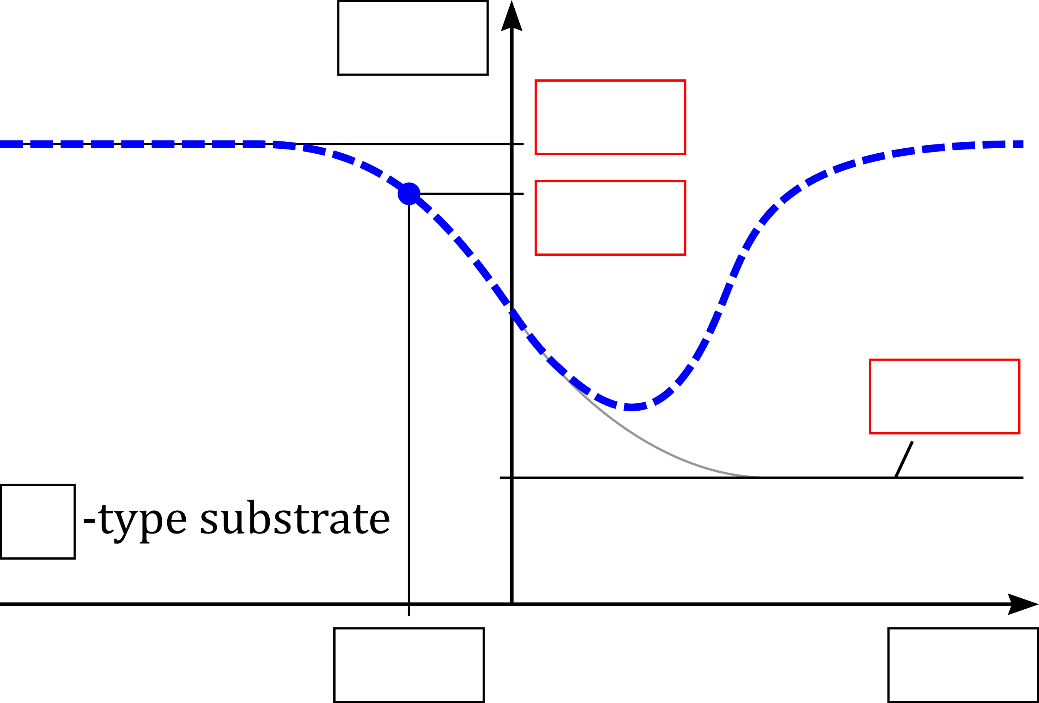
\includegraphics[width=0.66\textwidth]{figures/cv_fig3_blank.png}};
\begin{scope}[x={(img.south east)},y={(img.north west)}]
  \node at (0.385,0.955) {\small $C'$};
  \node at (0.585,0.840) {\scriptsize $C'_{\max}\!=\!C_{ox}$};
  \node at (0.585,0.695) {\scriptsize $C'_{FB}$};
  \node at (0.905,0.445) {\scriptsize $C'_{\min}$};
  \node at (0.035,0.280) {\small $p$};
  \node at (0.385,0.060) {\small $V_{FB}$};
  \node at (0.915,0.060) {\small $V_G$};
\end{scope}
\end{tikzpicture}

\caption{Assignment Figure~3 with the gaps filled in: $p$-type substrate, $y$-axis $C'$ and $x$-axis
$V_G$, the flat-band voltage $V_{FB}$, and the three red parameters $C'_{\max}=C_{ox}$, $C'_{FB}$ and
$C'_{\min}$.}
\label{fig:cv-annot}
\end{figure}

\textbf{(i) Values at \SI{300}{\kelvin}} (SiO$_2$, $\epsilon_r=3.9$, $t_{ox}=\SI{30}{\nm}$;
Si, $\epsilon_r=11.7$, $N=\SI{3e16}{\per\cubic\cm}$). All values per unit area:
\[
C'_{ox}=\frac{\epsilon_{ox}}{t_{ox}}=\SI{1.15e-3}{\farad\per\square\meter}\;(\SI{115}{\nano\farad\per\square\cm}).
\]
The bulk potential is $\phi_F=\tfrac{k_BT}{e}\ln\!\tfrac{N}{n_i}=\SI{0.375}{\volt}$, giving a maximum
depletion width
$W_{\max}=\sqrt{4\epsilon_{Si}\phi_F/(eN)}=\SI{180}{\nm}$ and Debye length
$L_D=\sqrt{\epsilon_{Si}(k_BT/e)/(eN)}=\SI{23.6}{\nm}$. With
$C'_{\min}=C_{ox}C_{sc}/(C_{ox}+C_{sc})$ for each series semiconductor capacitance:
\begin{center}\small
\begin{tabular}{lccc}
\toprule
Gate / doping & $C'_{\max}=C_{ox}$ & $C'_{FB}$ & $C'_{\min}$ \\
 & [nF/cm$^2$] & [nF/cm$^2$] & [nF/cm$^2$] \\
\midrule
SiO$_2$, $N=3{\times}10^{16}$ & 115 & 91 & 38.4 \\
\bottomrule
\end{tabular}
\end{center}

\textbf{(ii) Si$_3$N$_4$ gate ($\epsilon_r=7.5$) and lower doping $N=\SI{0.5e16}{\per\cubic\cm}$.}
The higher-$\kappa$ oxide nearly doubles $C_{ox}$, and the lighter doping widens the depletion region
($W_{\max}=\SI{413}{\nm}$), lowering $C'_{\min}$:
\begin{center}\small
\begin{tabular}{lccc}
\toprule
Gate / doping & $C'_{\max}$ & $C'_{FB}$ & $C'_{\min}$ \\
 & [nF/cm$^2$] & [nF/cm$^2$] & [nF/cm$^2$] \\
\midrule
Si$_3$N$_4$, $N=0.5{\times}10^{16}$ & 221 & 99 & 22.6 \\
\bottomrule
\end{tabular}
\end{center}
The capacitance swing grows from $C_{\max}-C_{\min}=\SI{77}{\nano\farad\per\square\cm}$ to
\SI{199}{\nano\farad\per\square\cm}, a factor of $2.6$. With $\Delta V$ fixed, the slope
$\Delta C/\Delta V$ therefore rises by the same factor, so the change makes a
\textbf{more sensitive sensor}.

\paragraph{Task 4 b) C--V modifications (low frequency).}
The flat-band voltage is
$V_{FB}=\tfrac{\phi_M}{e}-\tfrac{\phi_{Si}}{e}-\tfrac{Q_{ox}+Q_{ss}}{C_{ox}}$ (EOS adds
$E_{REF}-\psi_0+\chi_{sol}$). Each effect shifts the curve horizontally without changing its shape
(Fig.~\ref{fig:cv-mods}):
\begin{itemize}[nosep,leftmargin=1.4em]
\item \textbf{(i)} Fixed positive $Q_{ox},Q_{ss}$ lower $V_{FB}$ $\Rightarrow$ shift to the
\textbf{left} (negative $V$).
\item \textbf{(ii)} A higher semiconductor work function $\phi_{Si}$ also lowers $V_{FB}$
$\Rightarrow$ shift \textbf{left}.
\item \textbf{(iii)} Increasing pH makes $\psi_0$ more negative, and since $V_{FB}$ contains
$-\psi_0$ the curve shifts to the \textbf{right} ($\le\SI{59}{\milli\volt}/\mathrm{pH}$).
\end{itemize}

\begin{figure}[H]
\centering
% Auto-generated: TikZ overlay on the real docx Figure 4 (Task 4b)
\begin{tikzpicture}
\node[anchor=south west,inner sep=0] (img) at (0,0)
  {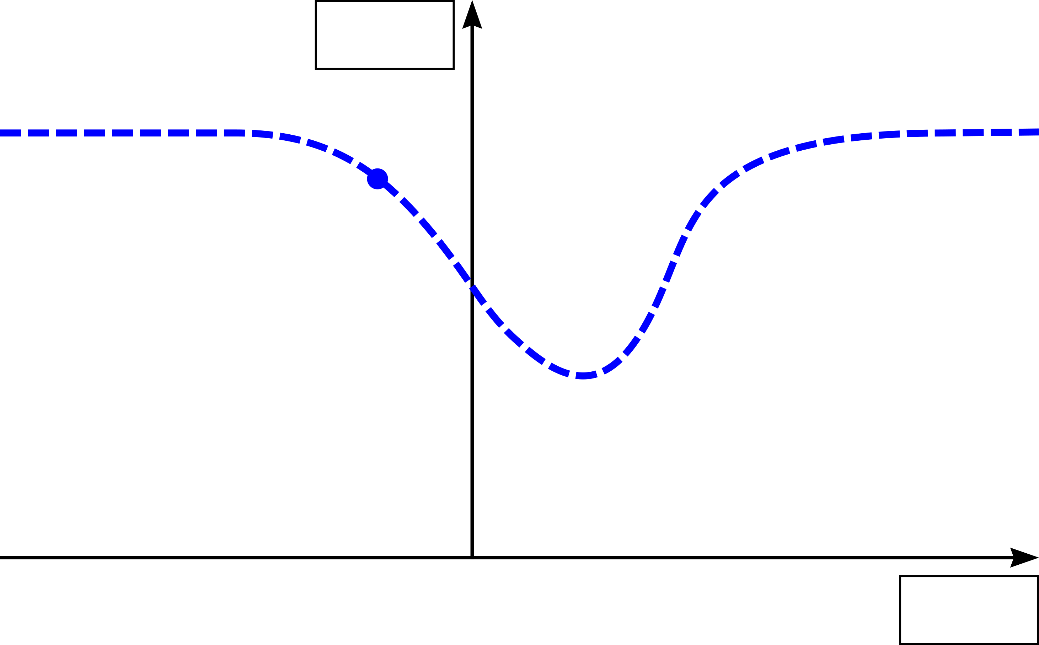
\includegraphics[width=0.66\textwidth]{figures/cv_fig4_blank.png}};
\begin{scope}[x={(img.south east)},y={(img.north west)}]
  \clip (0.0,0.13) rectangle (1.0,0.97);
  \draw[red,dashed,line width=1.1pt] plot coordinates {(0.000,0.795) (0.029,0.795) (0.059,0.795) (0.096,0.795) (0.125,0.794) (0.154,0.788) (0.182,0.777) (0.209,0.759) (0.234,0.729) (0.257,0.705) (0.281,0.671) (0.304,0.622) (0.328,0.572) (0.351,0.517) (0.374,0.478) (0.398,0.445) (0.424,0.423) (0.452,0.420) (0.481,0.455) (0.504,0.505) (0.527,0.586) (0.550,0.665) (0.575,0.716) (0.601,0.743) (0.629,0.763) (0.657,0.775) (0.686,0.784) (0.715,0.789) (0.745,0.793) (0.782,0.795) (0.812,0.795) (0.842,0.795) (0.871,0.796) (1.000,0.796)};
  \draw[green!55!black,dash dot,line width=1.1pt] plot coordinates {(0.000,0.795) (0.030,0.795) (0.059,0.795) (0.089,0.795) (0.119,0.795) (0.156,0.795) (0.185,0.794) (0.214,0.788) (0.242,0.777) (0.269,0.759) (0.294,0.729) (0.317,0.705) (0.341,0.671) (0.364,0.622) (0.388,0.572) (0.411,0.517) (0.434,0.478) (0.458,0.445) (0.484,0.423) (0.512,0.420) (0.541,0.455) (0.564,0.505) (0.587,0.586) (0.610,0.665) (0.635,0.716) (0.661,0.743) (0.689,0.763) (0.717,0.775) (0.746,0.784) (0.775,0.789) (0.805,0.793) (0.842,0.795) (0.872,0.795) (0.902,0.795) (0.931,0.796) (1.000,0.796)};
  \draw[violet,densely dotted,line width=1.1pt] plot coordinates {(0.000,0.795) (0.120,0.795) (0.150,0.795) (0.180,0.795) (0.210,0.795) (0.239,0.795) (0.269,0.795) (0.299,0.795) (0.336,0.795) (0.365,0.794) (0.394,0.788) (0.422,0.777) (0.449,0.759) (0.474,0.729) (0.497,0.705) (0.521,0.671) (0.544,0.622) (0.568,0.572) (0.591,0.517) (0.614,0.478) (0.638,0.445) (0.664,0.423) (0.692,0.420) (0.721,0.455) (0.744,0.505) (0.767,0.586) (0.790,0.665) (0.815,0.716) (0.841,0.743) (0.869,0.763) (0.897,0.775) (0.926,0.784) (0.955,0.789) (0.985,0.793) (1.000,0.793)};
  \draw[red,-{Latex},line width=0.9pt] (0.40,0.66)--(0.31,0.66);
  \draw[violet,-{Latex},line width=0.9pt] (0.62,0.66)--(0.71,0.66);
\end{scope}
\begin{scope}[x={(img.south east)},y={(img.north west)}]
  \node at (0.37,0.915) {\small $C$};
  \node at (0.93,0.05) {\small $V_G$};
\end{scope}
\end{tikzpicture}

\caption{Sketched over assignment Figure~4 (blue = ideal). \textcolor{red}{(i) red, dashed}: positive
fixed charge shifts left; \textcolor{green!55!black}{(ii) green, dash-dot}: higher work function
shifts left; \textcolor{violet}{(iii) violet, dotted}: increased pH shifts right.}
\label{fig:cv-mods}
\end{figure}

\paragraph{Task 4 c) EOS-Cap pH sensitivity.}
In the linear regime the chemical sensitivity is the product of the (shared) electrical slope and the
voltage shift per pH, $\Delta C/\Delta\mathrm{pH}=(\Delta C/\Delta V)\,(\Delta V/\Delta\mathrm{pH})$,
with the Nernst limit $\Delta V/\Delta\mathrm{pH}=2.303\tfrac{k_BT}{e}\,\alpha=\SI{59.5}{\milli\volt}\,\alpha$:
\[
\text{A (SiO}_2,\ \alpha=0.5):\ \frac{\Delta V}{\Delta\mathrm{pH}}=\SI{29.8}{\milli\volt}/\mathrm{pH},\qquad
\text{B (Al}_2\text{O}_3,\ \alpha=0.9):\ \frac{\Delta V}{\Delta\mathrm{pH}}=\SI{53.6}{\milli\volt}/\mathrm{pH}.
\]
Because both devices share the same slope $\Delta C/\Delta V$, their capacitive sensitivities scale
the same way: $\boxed{\,(\Delta C/\Delta\mathrm{pH})_B/(\Delta C/\Delta\mathrm{pH})_A=\alpha_B/\alpha_A=1.8\,}$.
The near-Nernstian Al$_2$O$_3$ device is $1.8\times$ more sensitive than the sub-Nernstian SiO$_2$ one.

\paragraph{Task 4 d) Effect of a different semiconductor.}
The pH response lives at the \emph{oxide--electrolyte} interface (it is set by $\psi_0$ and the
site-dissociation chemistry), so the intrinsic sensitivity in mV/pH does \textbf{not} change with the
semiconductor. What does change is the baseline: a different work function $\phi_{Si}$, bandgap, $n_i$
and permittivity shift $V_{FB}$ and reshape the C--V curve (different $C_{\min}$, depletion width) and
alter temperature stability and leakage. In short, the curve moves and rescales, but the pH
slope stays the same.

\section*{Part E: Introduction to FEM (Unit 5)}
\addcontentsline{toc}{section}{Part E: Introduction to FEM}

\paragraph{1. Three key steps from physics to a numerical discretization.}
\begin{enumerate}[nosep,leftmargin=1.6em]
\item \textbf{Mathematical model (strong form).} Capture the physics as a governing PDE plus its
boundary and initial conditions: the exact, continuous description.
\item \textbf{Weak / variational form.} Multiply by a test function and integrate over the domain,
moving derivatives onto the test function. This relaxes the continuity requirement and is what makes
the problem amenable to piecewise approximation.
\item \textbf{Discretization (Galerkin).} Mesh the domain into finite elements, expand the unknown in
a finite set of basis (shape) functions, and assemble the result into an algebraic system
$\mathbf{K}\mathbf{u}=\mathbf{f}$ that a computer solves; then post-process and check convergence.
\end{enumerate}

\paragraph{2. Ideal polynomial order of the basis functions.}
\textbf{Quadratic (second-order) elements} are usually the sweet spot.
\begin{itemize}[nosep,leftmargin=1.6em]
\item \emph{Lower order} (linear/hat functions) is cheap and robust and represents straight fields
exactly, but it only captures curvature crudely, so smooth or high-gradient fields need a very fine
mesh to reach the same accuracy.
\item \emph{Higher order} (cubic and up) gives excellent accuracy per element and resolves curvature
with few elements, but the cost per element climbs, matrices become denser and worse-conditioned, and
high orders can oscillate (Runge-type wiggles) near sharp features.
\end{itemize}
Quadratic elements capture curvature well while keeping the cost and conditioning manageable, which
gives the best accuracy per unit effort for typical smooth problems.

\paragraph{3. Qualitative grid spacing for linear (hat) basis functions.}
Linear hat functions reproduce a straight line \emph{exactly}, so the rule is simple: \textbf{use a
coarse spacing on straight parts, refine where the curvature is high, and always place a node at every
corner/kink} (where the slope is discontinuous).
\begin{itemize}[nosep,leftmargin=1.6em]
\item \textbf{(a) Straight line:} one element (two nodes) is enough, since it is exact.
\item \textbf{(b) Exponential:} a graded mesh, fine where the function bends sharply and progressively
coarser in the flat tail.
\item \textbf{(c) Mixed curve:} coarse on the straight segments and the triangular peak (with nodes at
the joints $x=-4,-2,2,4,6$), but densely spaced across the high-curvature semicircle.
\end{itemize}

\begin{figure}[H]
\centering
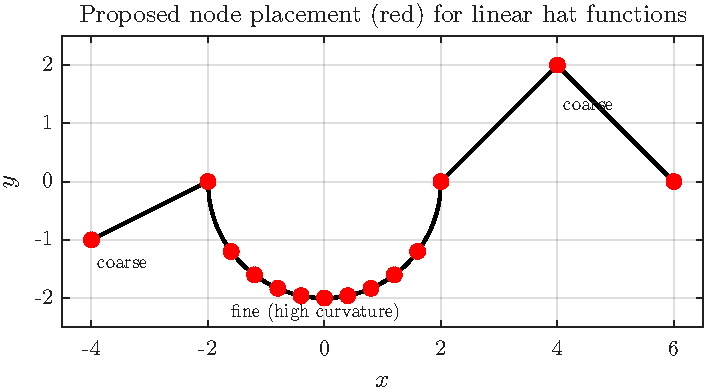
\includegraphics[width=0.66\textwidth]{figures/fem_grid.pdf}
\caption{Proposed node placement (red) for curve (c): coarse on the straight pieces, dense across the
curved semicircle, with nodes pinned at every kink.}
\label{fig:femgrid}
\end{figure}


\end{document}
